\documentclass{standalone}
\usepackage{tikz}


\begin{document}

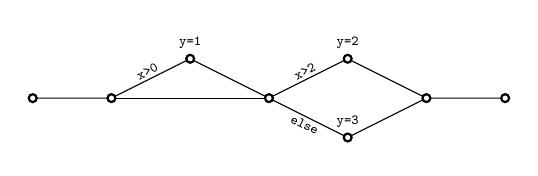
\begin{tikzpicture}[sequence point/.style={thick,fill=white},
                    execution path/.style={thin}]
  \draw[execution path] (0,0) -- (1,0) -- (2,.5) node[midway,sloped,yshift=1mm] {\tiny\tt x>0} -- (3,0) -- (4,.5) node[midway,sloped,yshift=1mm] {\tiny\tt x>2} -- (5,0) -- (6,0);
  \draw[execution path] (1,0) -- (3,0);
  \draw[execution path] (3,0) -- (4,-.5) node[midway,sloped,yshift=-1mm] {\tiny\tt else} -- (5,0);

  \draw[sequence point] (0,0) circle (.05);
  \draw[sequence point] (1,0) circle (.05);
  \draw[sequence point] (2,.5) circle (.05) node[above] {\tiny\tt y=1};
  \draw[sequence point] (3,0) circle (.05);
  \draw[sequence point] (4,.5) circle (.05) node[above] {\tiny\tt y=2};
  \draw[sequence point] (4,-.5) circle (.05) node[above] {\tiny\tt y=3};
  \draw[sequence point] (5,0) circle (.05);
  \draw[sequence point] (6,0) circle (.05);
\end{tikzpicture}

\end{document}